
% This template has been edited from the IEEE template available at:
% https://www.ieee.org/conferences/publishing/templates.html
%
% For further help, you may wish to see:#

% https://www.overleaf.com/learn/latex/tables
% https://www.overleaf.com/learn/latex/Inserting_Images
% https://www.overleaf.com/blog/532-creating-and-managing-bibliographies-with-bibtex-on-overleaf

\documentclass[conference]{IEEEtran}
%\IEEEoverridecommandlockouts
% The preceding line is only needed to identify funding in the first footnote. If that is unneeded, please comment it out.
\usepackage[a4paper, total={6in, 8in}, margin=0.75in]{geometry}
\usepackage{cite}
\usepackage{amsmath,amssymb,amsfonts}
%\usepackage{algorithmic}
\usepackage{algorithm} 
\usepackage{algpseudocode} 
\usepackage{graphicx}
\usepackage{appendix}
\usepackage{textcomp}
\usepackage{xcolor}
\usepackage{bm}
\def\BibTeX{{\rm B\kern-.05em{\sc i\kern-.025em b}\kern-.08em
    T\kern-.1667em\lower.7ex\hbox{E}\kern-.125em}}
\begin{document}

\title{Report Title: Be Descriptive}

\author{
    \IEEEauthorblockN{Student Number}
    \and
    \IEEEauthorblockN{Student Number}
}

\maketitle

\begin{abstract}
%最后写摘要是正常的。  
%首先,尽量简明扼要地说明所调查的问题/疑问/挑战。  
%第二,说明你发现了什么。  摘要应该帮助读者决定他们是否有兴趣阅读整篇论文。  
% 本文基于Pololu 3pi+ 32U4 robot研究了PID控制器性能与其update frequency的关系。我们在2-500的频率范围内进行了多次实验,总结了变化的规律,最终发现高频和低频都会使PId的控制性能降低,对于实验中的被控对象,40-120是性能最佳的频率范围。
In this paper we investigated the relationship between PID controller performance and its update frequency based on the Pololu 3pi+ 32U4 robot. We conducted several experiments in the frequency range of 2\bm{$\sim$}500 and summarised the pattern, eventually finding that both high and low frequencies degrade the control performance of the PID controller, and that 40\bm{$\sim$}120 is the best frequency range for the performance of the object being controlled in the experiments.
\end{abstract}


\section{Introduction}
\label{Introduction}
Proportional-integral-derivative (PID) control is the most commonly used control algorithm in the industry and has become universally accepted in industrial control\cite{knospe2006pid}. For autonomous robotic systems that can travel, 
% 对于任何需要追踪给定量的控制系统来说,PID都是非常重要的算法。通过PID算法,可以在没有系统精细数学模型的情况下,完成系统的无静差控制量追踪。所以,PID控制器的性能与参数的关系是一个实用且重要的研究方向。
PID is a important algorithm for any control system that needs to track a given amount of quantity. With the PID algorithm, it is possible to accomplish steady-state error free target tracking of a system without a fine-grained mathematical model of the system. Therefore, the performance of PID controllers in relation to parameters is an important research area and has strong integration with practical applications.
% PID控制的运算中包含时间变化,所以PID控制器的性能会受到其更新频率的影响。
PID control algorithm include time variation, so the performance of the PID controller is affected by its update frequency. Update frequency is a hidden parameter for PID controller other than the well-known $K_{p}$, $K_{i}$, and $K_{d}$. 
 If an optimum frequency range is found to improve the PID performance, this will provide a reference for future commissioning of other control systems to obtain better performance.

A typical PID step response\cite{goodwin2001control} is shown in Fig. \ref{PIDandSettlingTime}. The blue line in the figure shows the process of a PID controller tracking the target. % PID控制器的任务就是使蓝色线条(被控量)在一定时间内达到target值。对于这个控制过程,还有一些常见的性能衡量指标,如图中所示的overshoot,setting time等。我们会在23两节详细解释这部分内容。
The task of the PID controller is to make the blue line (the controlled value) reach the target value within a certain time. There are also some common performance metrics for this control process, such as overshoot, setting time, etc. shown in the 
 Fig. \ref{PIDandSettlingTime}. We will explain this part in more detail in following sections(\ref{Implementation}, \ref{Experiment Methodology}).
\begin{figure}[htbp]
\centerline{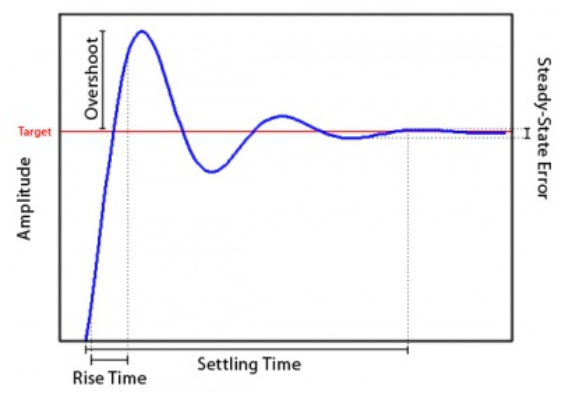
\includegraphics[width=0.9\linewidth]{Report/Pic/PIDandSettlingTime.png}}
\caption{Typical PID step response and PID performance metrics.}
\label{PIDandSettlingTime}
\end{figure}

\subsection{Hypothesis Statement}
% 我们的假设可以归纳为以下三句话:
Our hypothesis can be summarised as follows:
\begin{enumerate}
    \item High update frequency makes the PID controller changes can not be reflected in time on the controlled object, and reduce the performance.
    \item Low update frequency leads to a slow response speed\cite{knospe2006pid}, which affect real-time controlling and therefore controller performance.
    \item In the frequency range, there could be an optimal frequency band that can better balance all aspects of the PID to achieve better performance.
\end{enumerate}

To investigate our hypothesis, we implemented a basic PID controller based on Pololu 3pi+ 32U4 robot, designed a set of experiments, and \textbf{tested the relationship between the PID controller update frequency and it's performance}.
\subsection{Report Structure}
\begin{enumerate}
    \\\textbf{\ref{Introduction}. Introduction:} A brief introduction to our research topic and our hypothesis.
    \\\textbf{\ref{Implementation}. Implementation:} Introduction to the hardware system and control algorithms used for the experiments.
    \\\textbf{\ref{Experiment Methodology}. Experiment Methodology:} Details of the experiment procedures, the flow of the automatic experiment program, the variables involved in the experiments, and the metrics for performance evaluation.
    \\\textbf{\ref{Results}. Results:} The results observed in our experiment, from both the metrics and behind the metrics.
    \\\textbf{\ref{V_Discussion and Conclusion}. Discussion and Conclusion:} The significance of the experimental results for our hypothesis, the existing shortcomings in the experiment, and the direction of future work.
    
\end{enumerate}





\section{Implementation}
\label{Implementation}
% 2.
% 在这一节中,你应该描述你的实现的具体细节,以便你的读者可以重新创建你的工作。  
% 如果你使用了一个已经被广泛理解的算法或技术,你可以只参考一个外部来源而不详细解释,除非解释算法/技术为读者提供了关于你的项目的重要信息。 
% 你可能希望在这里介绍技术信息,以支持对特定组件的理解(例如,一个传感器或执行器的响应图,或者如果你在实验前有一个早期的可行性研究)。
% 如果你要将你的机器人系统与自己进行比较,那么你可能需要记录你的 "基础"解决方案和你的 "改进版"解决方案。  
In this paper we have measured the performance of the PID controller with the Pololu 3pi+ 32U4 robot. We implemented the robot's wheel motor control, wheel speed measurement and PID control of the wheel speed in software.
% 本文中,对PID控制器的性能是在Pololu 3pi+ 32U4 Robot身上展开的。我们用软件实现了机器人的轮子电机控制,速度追踪,以及对轮子速度的PID控制。

% 插入系统框图
\begin{figure}[htbp]
\centerline{\includegraphics[width=0.6\linewidth]{Report/Pic/ImplementFLowChart.png}}
\caption{System Components.}
\label{fig_ImplementFlowChart}
\end{figure}

% 系统主要有5个组成部分:PID控制器,Motor Driver,Wheel,Encoder, Kinematics
System has \textbf{4 main components: PID controller, wheel and motor driver, encoder, kinematics.} They are structured as shown in Fig. \ref{fig_ImplementFlowChart}. 
\begin{itemize}
    \item\textbf{PID Controller: } We use a basic PID controller in our system to minimise the number of irrelevant variables. We do not want popular improvements to the PID to become variables in the system, such as integral limitation. The PID controller we use can be described as below:
    
    
        \begin{equation}\label{PID_1}
            e(t) = r(t) - y(t)      
        \end{equation}
        $r(t)$: set point value, or say the aim of the system\\
        $y(t)$: system output \\
        $e(t)$: error
        \begin{equation}\label{PID_2}
            u(t)=K_{p}*e(t)+K_{i} * \sum_{i=1}^{k}  (e(t_{i})\Delta t)+K_{d} * \frac{de(t)}{dt}
        \end{equation}
        $u(t)$:PID controller output
        \par
    \item\textbf{Wheel and Motor Driver: }For Pololu 3pi+ 32U4 robot, user could control the motor speed by controlling motor PWM duty cycle ratio. Motor takes 0$\sim$255(integer) as input and output 0$\sim$5V power to drive the wheels. The relationship between wheel speed and PWM duty cycle is shown in Fig. \ref{fig_WheelCharacter}.
    %插入电机速度与输入的特性图 %
    % 也就意味着速度计算有一些误差(难以测得一圈的编码数),但速度误差对本文中的实验没有影响。
    \item\textbf{Encoder: }Each wheel shaft has an encoder that can be used to measure the movement of the wheel. Encoder counts between 358$\sim$359 for a 360° wheel spin. It also means that there is some error in the velocity calculations (it is no exact code count for one whole lap), but the velocity error has no effect on the experiments in this paper, for we are looking at relationships rather than specific values.
    % 用编码器值的变化与轮子的周长计算轮子的运动,藉此计算机器人kinematics。在本文中只需计算运动学中的轮子速度部分。
    \item\textbf{Kinematics: }The motion of the wheel is calculated using the variation of the encoder value with the circumference of the wheel in order to calculate the robot kinematics. In this paper only the wheel speed part of the kinematics is needed.

\end{itemize}

\begin{figure}[htbp]
\centerline{\includegraphics[width = \linewidth]{Report/Pic/WheelResponse.png}}
\caption{Diagram of wheel speed versus PWM value. Non-linear characteristics in the test range (speed around 1)} % 轮子速度与PWM值的关系
\label{fig_WheelCharacter}
\end{figure}



\section{Experiment Methodology}
\label{Experiment Methodology}
% 3.
% 在这一节中,记录你是如何组织(设计)你的实验的,从而使其他人可以很容易地重新创造你的工作。  
% 你也希望你的读者同意你仔细考虑了你的实验,这样我们就可以相信你的结果是有意义的,而且是可信的(没有错误)。 
% 你在这一节中使用哪些小节(如果有的话),主要取决于你的项目和你选择的展示方式。  以下是一些建议,以帮助你的工作清晰化。

To test our hypothesis, we investigated the effect of PID update frequency on the performance of the PID controller.

% 

\subsection{Overview of Method}
\label{PIDTuningMethod}
% 3.A
% 向读者描述你的实验的一般结构和程序。你应该提供一个有点像蛋糕食谱的规格。 
% 例如:你的实验持续多长时间? 你使用多少次重复试验?有多少种备用方案?
The main focus of the experiment was to \textbf{keep the PID parameters constant and change the update frequency of the PID controller to observe the change in performance metrics} (overshoot, setting time). A frequency range of \textbf{2Hz $\sim$ 500Hz} was selected for testing based on the actual control requirements and hardware performance limitations (outside of this range the controller output can oscillate violently). \textbf{Using the same set of PID parameters for the entire frequency range would produce oscillations at most of the tested frequencies and produce meaningless test data}, so we adopted the following approach: 
% 实验的主要内容就是保持PID参数不变,改变PID控制器的update freqeucy, 观察性能指标(overshoot, setting time)的变化。根据实际控制的需求和硬件性能的限制,我们选定2Hz~500Hz的频率范围来进行测试(在此范围外控制器输出会产生剧烈震荡)。对整个频率范围使用同一组PID参数会使大部分受试频率产生震荡,产生无意义的测试数据,因此我们采用这样的方法:

% 插入系统框图
\begin{figure}[htbp]
\centerline{\includegraphics[width=\linewidth]{Report/Pic/FrequencyRangeExplained.png}}
\caption{Method of iterating through the frequency range.}% 遍历频率域的方法
\label{fig_FrequencyRange}
\end{figure}

We select 15 frequencies ($f_{1}\sim f_{15}$) at equal distances in the range $[2,500]$,  and \textbf{for each frequency we tune a set of PID parameters. Parameter tuning follows a common principle:}
\begin{enumerate}
    \item\textbf{ Keep \bm{$K_{p}$} constant. }We found no observable effect of frequency change on the proportional part. Probably because the proportional part of the calculation does not involve a change in time.
    \item\textbf{ Keep overshoot \bm{$\leq10\%$}. }
    \item\textbf{ Ensure PID controller reaches steady-state within 6 updates.} This is not practical for high frequency, so for high frequencies we try to minimize setting time  while still meeting the requires above. 
\end{enumerate}

%接下来解释算法
% 对于f1-15中的每一个频率,我们都在其邻域中测试此频率所对应的PID参数的性能。取当前频率的前一个与后一个频率作为邻域的上下限(若没有前一个或后一个,则用自己代替)。在邻域中取十个等间距点,测试PID控制器的性能。

For each frequency $f_{i}$ in $f_{1}\sim f_{15}$, we test the PID controller performance in its neighbourhood,with the PID parameter tuned for $f_{i}$. The previous frequency ($f_{i-1}$) and next frequency ($f_{i+1}$) to the current frequency are taken as the upper and lower limits of the neighbourhood (if there is no previous or next, use $f_{i}$ instead). 10 equally spaced points in the neighbourhood are taken to test the performance of the PID controller.

\begin{algorithm}
	\caption{Test Process}\label{TestMethod}
	\begin{algorithmic}[1]
        \State Calculate 15  equidistant frequencies $f_{1}\sim f_{15}$ in range of $[2,500]$
	\For {$f_{i}=f_{1},f_{2},\ldots,f_{15},$} 
                \State Tune PID parameters $K_{i}$, $K_{d}$ for $f_{i}$
                \State Calculate 10 equidistant frequencies $f_{n1}\sim f_{n10}$ in range of $f_{i}$'s neighbourhood $[f_{i-1},f_{i+1}]$
                \State In 4: if $i-1<0$ or $i+1>15$, use $f_{i}$ instead
			\For {$f_{n}= f_{n1},f_{n2},\ldots,f_{n10}$}
				\State Use step signal as left wheel speed set point
                \State Measure PID performance with step response
                \State Calculate the \textbf{mean} overshoot and setting time of \textbf{10 responses}
                \If{Controller failed to reach steady-state within \textbf{1 second}} Return a NaN value which represents system oscillate        
                \EndIf
			\EndFor
		\EndFor
	\end{algorithmic} 
\end{algorithm}

% 整个实验除PID参数为预先调节并储存好以外,均为自动进行。最大程度减少了人为干预。
 \textbf{The entire experiment is carried out automatically,} except for the PID parameters, which are pre-adjusted and stored. \textbf{Human intervention is minimised. The code we use has been shared on GitHub.} 
 
% 我们使用邻域来进行测试,是为了在保证PID控制器稳定(来获得有意义的结果)的同时,展示不同频段上频率变化对PID控制器性能的影响。
We use neighbourhoods to perform the test in order to demonstrate the effect of frequency variations on the performance of the PID controller over different frequency ranges while ensuring that the PID controller is stable (to obtain meaningful results).

\subsection{Discussion of Variables}
\label{DiscussionOfVariables}
% 3.B
% 你应该概述一下你的实验中的关键变量。这将有助于你的读者以后相信你的结果是可信的,而不会读不懂。
Variables in this experiment are: \bm{$K_{p}$}, \bm{$K_{i}$}, \bm{$K_{d}$}, PID update frequency \bm{$f$}, left wheel speed set point \bm{$v$}.
\begin{itemize}
    % 变量表
    % 受控变量:这些是你的实验(任务、硬件、软件、环境)的部分,这些部分可能会有变化,但你通过仔细设计实验来控制它们。例如,电池寿命不同,所以你将使用新电池。
    \item \textbf{Controlled Variables}: 
        \begin{itemize}
            \item Robot related variables: We use new battery for tests, also flip robot over during the whole test, make sure it's left wheel is free to spin and not blocked.
            \item PID parameter \bm{$K_{p}$}: We use the same $K_{p}$ during the whole test, for we didn't find observable difference in PID proportion part.
            \item Left wheel speed set point \bm{$v$}: We set it 1.00(m/s) as the given aim for PID controller.
        \end{itemize}
    % 自变量:这是你要改变的实验部分,以便你希望观察到性能的可测量的改变。  请注意,我们曾经只想要一个自变量--有时我们以此为目标,但承认其他部分会发生变化,我们需要对我们的系统和/或结果进行仔细分析。
    \item \textbf{Independent Variable}: 
        \begin{itemize}
            \item PID update frequency \bm{$f$}: We change the frequency across the whole range as previously described. 
            \item PID parameter \bm{$K_{i}$} and \bm{$K_{d}$}: For each neighborhood we use a unique set of PID parameters, to keep PID stable at different frequencies. Since we are looking at the effect of frequency shift on performance in the same neighbourhood, these variable have no affect on the experimental results. 
        \end{itemize}
    % 因变量:这些是你的实验的一部分,你希望在其中观察到一个可测量的变化。  你将设计或选择适当的参数来测量和分析这个可依赖的变量。  例如,我们可以有一个系统的因变量,但使用平均值、模式和中位数的指标来分析它。
    \item \textbf{Dependent Variable(s)}:  all metrics are \textbf{measured and calculated automatically by experiment program}.
        \begin{itemize}
            \item Overshoot(\%): The amount that the process variable overshoots the final value, expressed as a percentage of the final value.
            \item Setting time(ms): If process variable shows three consecutive points are within $\pm5\%$ error of the final value, the system is considered stable and the setting time is recorded.
            % 如果有连续三个点在给定值±5%范围内,则判定系统稳定,记录稳定时间
        \end{itemize}
\end{itemize}

\subsection{Discussion of Metrics}
\label{Metrics}
% 3.C 讨论参数
% 在这一部分,你应该讨论你选择指标的理由(为什么)--例如,这些指标如何帮助我们解释你的结果?  你的衡量标准需要在整个实验中得到一致的应用,以便提供性能的比较。  
% 你应该讨论你的衡量标准的优点和缺点。  通常,我们需要一个以上的指标来弥补另一个指标中被混淆或隐藏的信息。  通过使用一个以上的指标,我们可以更接近于你的实验结果的真相。  

% 我们所使用的overshoot和setting time是经典的PID性能指标。我们放弃rise time和steady-state error是因为(1)我们观察到很多时候PID控制器第一次update就会产生overshoot,没有rise的过程。(2)在本实验中steady-state error有一点被customized setting time 覆盖了。且steady-state error往往很小,观测意义不大
The overshoot and setting time that we use are classical PID performance metrics. We do not use rise time and steady-state error because \textbf{(1)} We observe that many times the PID controller produces overshoot on the first update and there is no rise process. \textbf{(2)} In this experiment the steady-state error is partially covered by the customised setting time. And the steady-state error is often so small that the observation is not of much significance. Also note that the setting time we use is customized for programming.

For a discrete controller, it may be unfair to use setting times (ms) to evaluate system performance at all frequencies, as lower frequencies naturally have longer setting times. 



\section{Results}
\label{Results}
% 4.
% 在这一部分中,你应该介绍你的结果。 
% 一般来说,最好是既要有 "定量 "的结果(如数据),又要有 "定性 "的结果(如有代表性的书面观察或图表)。  
% 你应该在有助于清晰的地方使用分节。 
% 例如,先介绍 "基础"系统的结果,然后介绍 "改进后"系统的结果,最后介绍同时考虑 "基线 "和 "改进 "系统的结果,这可能是有用的。  
% 然而,这将完全取决于你的项目和你如何设计你的实验。
% 在介绍结果时,应力求在介绍中清楚地传达一种见解。
% 例如,一张包含所有单个数据的大表需要读者做大量的工作来找出重要的内容。 
% 与此相反,一个适当展示平均数和标准差的表格已经为读者总结了结果(而且会更有用)。  
% 同样,在可能的情况下,将数据合并到图表中,以便进行直接比较--在可能的情况下,包括误差条。  

% 克制自己,有的东西不该在这里讨论。而应该在v中详细介绍
\subsection{Overview of Results}
% 实验的总体结果详见附录中的的图(引用)。根据PID控制器性能的变化,我们将完整的频率范围分为三个频段:低频(0,40),中频(40,230),高频(230,500)。接下来展示PID控制器的性能在这三个频段中发生的变化。
The overall results of the experiment are detailed in the figure in the appendix (Fig. \ref{fig_appendix}.). \textbf{The complete frequency range was divided into three bands according to the variation in the performance of the PID controller: low frequency \bm{$f=[0,40]$}, medium frequency \bm{$f=[40,230]$}, and high frequency \bm{$f=[230,500]$}}. The next subsection shows how the performance of the PID controller changes over these three frequency bands.
\subsection{Result Details (Fig. \ref{fig_LowFrequency}, \ref{fig_MediumFrequency}, \ref{fig_HighFrequency}.) } 
    \textbf{Graph explanation:} Each line in the graph represents a neighbourhood with its corresponding PID parameter set to show the PID performance at different frequencies. The red dot at the bottom represents where the process value oscillates and fails to reach steady-state. Labels show the center frequencies of each neighbourhood.
% 图中的每条线代表一个邻域与其对应的PID参数在不同频率下展现的PID性能。底部的红点代表在此处被控量震荡而不能达到稳态。
        \begin{figure*}
            \centering
            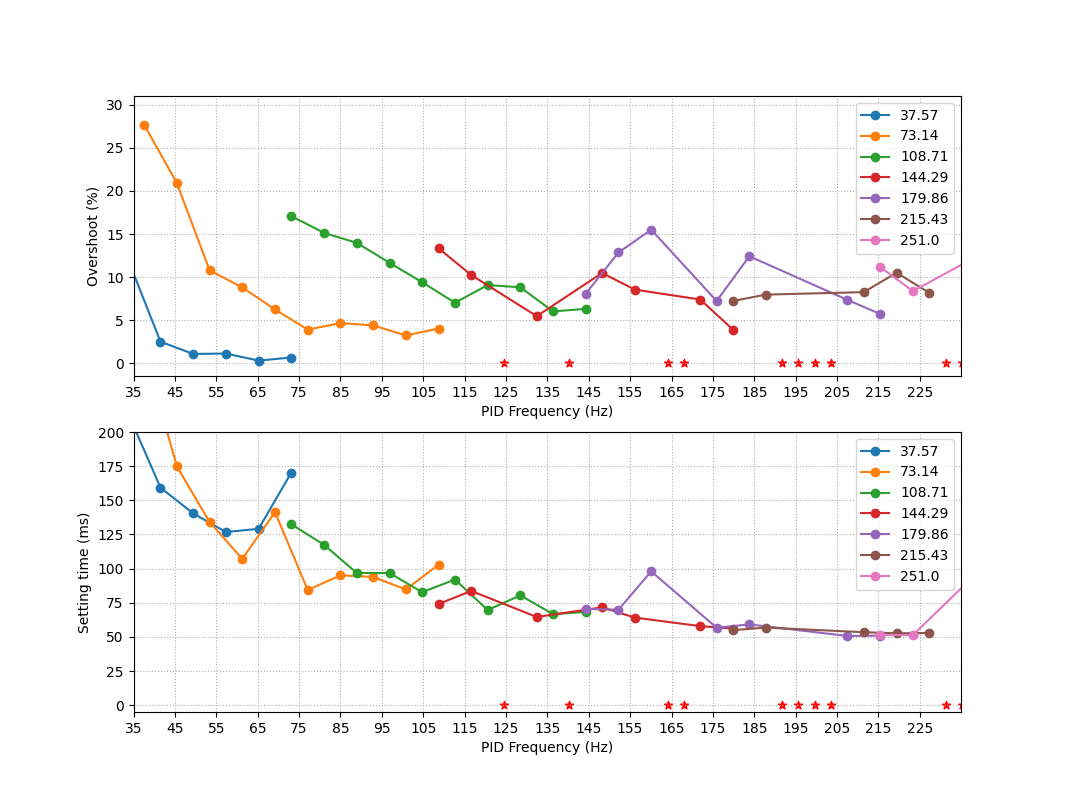
\includegraphics[width=0.8\linewidth]{Report/Pic/ResultMediumFrequency_2.png}
            \caption{Medium update frequency PID performance.}
            \label{fig_MediumFrequency}
        \end{figure*}
        \begin{figure}[htbp]
        \centerline{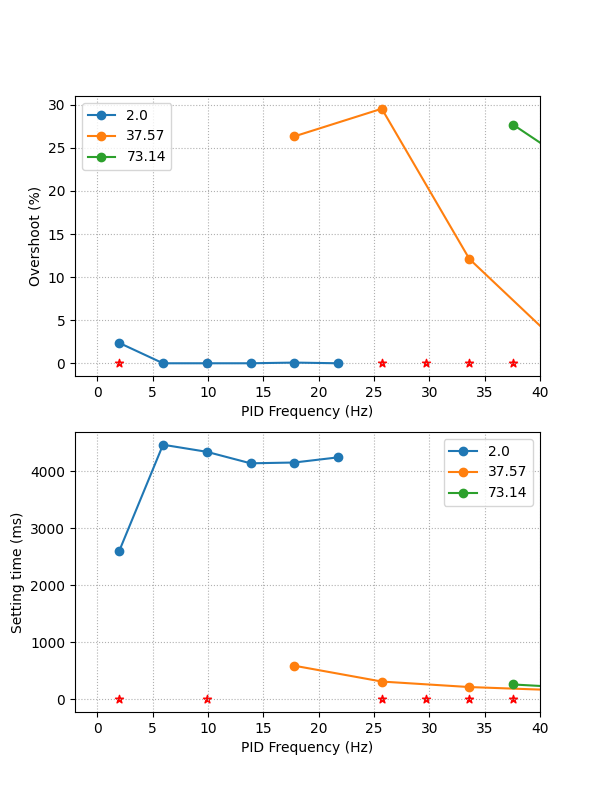
\includegraphics[width=\linewidth]{Report/Pic/ResultLowFrequency_2.png}}
        \caption{Low update frequency PID performance.}
        \label{fig_LowFrequency}
        \end{figure}
        \begin{figure}
            \centering
            \includegraphics[width=1.05\linewidth]{Report/Pic/ResultHighFrequency.png}
            \caption{High update frequency PID performance.}
            \label{fig_HighFrequency}
        \end{figure}
\begin{itemize}
    \item \textbf{Low Frequency(\bm{$f=[0,40]$}):} Fig. \ref{fig_LowFrequency}.
        %超调和调节时间最大。其中,调节时间明显比其他频段更长。随着频率上升,系统的调节时间和超调展现出逐渐减小的趋势。图右侧的四个红点是2邻域最右侧点发生震荡,左侧的两个红点是37.57邻域的最左侧两个点发生震荡。 
        \\Overshoot and setting times are the largest. \textbf{The setting time is significantly longer than in the other frequency bands. As the frequency increases, the setting time and overshoot of the system show a decreasing trend.} The four red dots on the right side of the graph are the rightmost points of the $f=2$ neighbourhood where oscillation occurs, and the two red dots on the left side are the leftmost two points of the $f=37.57$ neighbourhood where oscillation occurs. 
    \item \textbf{Medium Frequency(\bm{$f=[40,230]$}):} Fig. \ref{fig_MediumFrequency}.
        %PID控制器在此频段中性能最好。有最低的超调和调节时间。性能仍然随频率上升而改善。注意,随着频率上升,开始出现一些离散的易震荡频段,在这些频段中PID控制器突然变得非常容易震荡。这样的易震荡频段随频率上升而增多。图中所有的离群点都是位于震荡频段边缘的点。
        \\The PID controller has the best performance in this frequency band. There is the lowest overshoot and setting time. Performance still improves with increasing frequency. Note that as frequency rises, some discrete oscillation-prone bands begin to appear where the PID controller suddenly becomes very oscillatory. Such oscillation-prone bands increase with increasing frequency. \textbf{All the outliers in the graph are points at the edges of the oscillatory bands.}
    \item \textbf{High Frequency(\bm{$f=[230,500]$}):} Fig. \ref{fig_HighFrequency}.
    \\
    % 性能开始随频率的上升而下降。超调量和调节时间都开始逐渐上升。同时,此频段的震荡频段进一步增加,大多频率点都发生了震荡。但这种震荡与低频段的震荡是不同的,这种震荡更多代表的是稳态的不稳定。我们在后面详聊。
    The performance starts to \textit{decrease} as the frequency rises. Both the overshoot and the setting time begin to rise gradually. At the same time, the oscillation band in this frequency band increases further, with oscillation occurring at most frequency points. However, this oscillation is different from the oscillation in the low frequency bands. Such oscillation represents more of a steady-state instability. We describe this in subsection \ref{BehindMetrics}.
\end{itemize}
\subsection{Other than Metrics}
\label{BehindMetrics}
% 震荡
% PID参数变化趋势
% 高速时运动学计算比轮子旋转快的问题
% 震荡频段
\begin{itemize}
    \item \textbf{Two Kinds of Oscillations:}\\
        % 高频段的震荡和低频段的震荡是不同的。根据我们的定义:如果没能在一秒内保持连续三次稳定在If process variable failed to show three consecutive points are within $\pm5\%$ error of the final value in 1 second period, the system is considered oscillate. 但有两种情形符合这一定义:1)被控量在给定值上下大幅度震荡(一般意义上的震荡) 2)稳态性能太差,稳态误差无法维持在±5%的范围内,被判定为震荡。在我们的实验中,低频段的震荡属于前者,而高频段的震荡属于后者。即,低频时控制器使系统被控量上下大幅度震荡,高频时系统给定值的附近持续小幅度震荡,且此种震荡不能保持在±5%误差范围内。
        \textbf{Oscillations in the high frequency band are different from oscillations in the low frequency band.} According to our definition: if the process variable fails to show three consecutive points are within $\pm5\%$ error of the set point in 1 second period, the system is considered oscillate. However, there are two cases that fit this definition:
        \begin{enumerate}
            \item The process variable oscillates significantly above and below the given value (oscillation in the general sense).
            \item The steady state performance is so poor that the steady state error cannot be maintained within $\pm5\%$ and is judged to be oscillate.
        \end{enumerate}
       In our experiments, oscillations in the low frequency band fall into the former category, while oscillations in the high frequency band fall into the latter category. \textbf{That is, at low frequencies the controller causes the system to oscillate up and down significantly, and at high frequencies the system oscillates continuously in small ranges around  set point, and this oscillation cannot be maintained within $\pm5\%$ error.}
    \item \textbf{Trends in PID Parameters: Fig. \ref{KiTrend}}\\
    % 在我们为频率范围内的点调节PID参数时,我们观察到了以下特点:
    When we tuned the PID parameters (see \ref{PIDTuningMethod}) for points in the frequency range, we observed the following characteristics:
    \begin{enumerate}
        % Ki: 从极低(0.045)开始,随频率上升而增加,在f=322.1处突然减小,但仍保持与频率的正相关。
        % Ki: 从极高(0.045)开始,随频率上升而增加,在f=322.1处突然减小,然后保持不变。
        \item \bm{$K_{i}$}: Starting at a very low value (0.045) and increasing with frequency, it suddenly decreases at $f = 322.1$, but still maintains a positive correlation with frequency.
        \item \bm{$K_{d}$}: Starting at a outlier high value (1000.00 at $f=2.00Hz$) and decreasing with frequency, it suddenly increases at $f = 322.1$, and remains stable (i.e., in our test, $K_{d}$ has little influence to performance in high frequency band).
        \begin{figure}
            \centering
            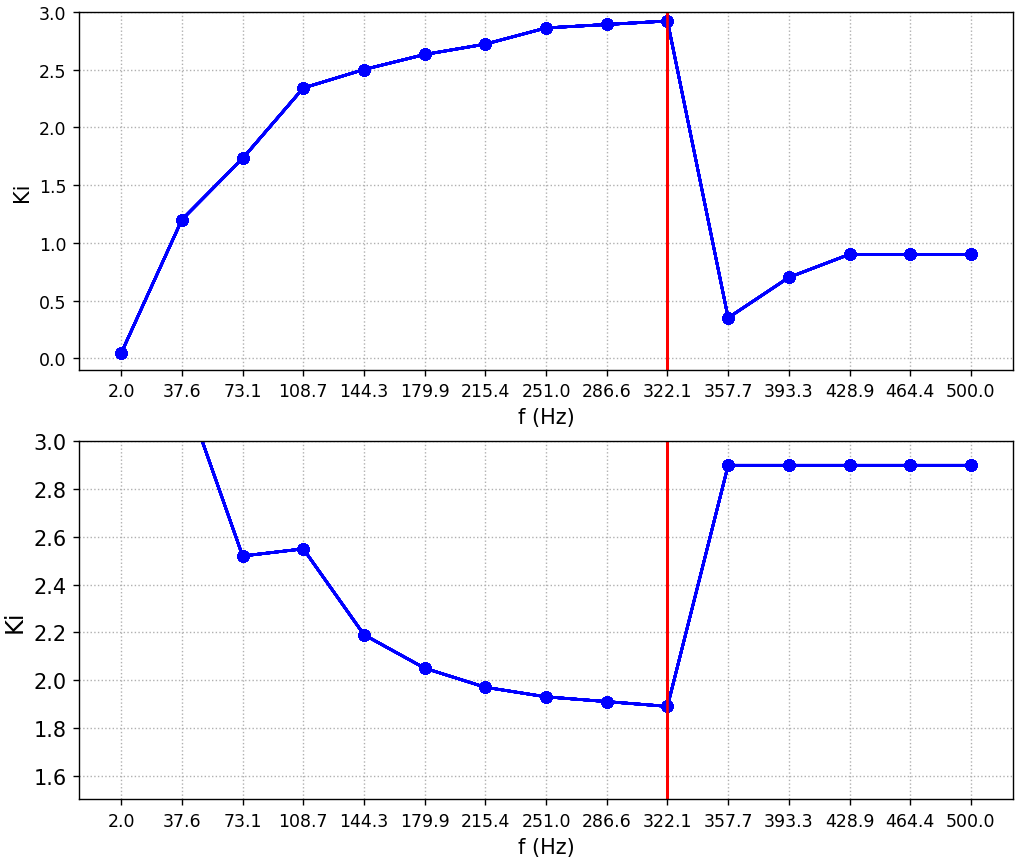
\includegraphics[width=1.1\linewidth]{Report/Pic/KiKdTrend.png}
            \caption{PID parameters trend. \textbf{Red line marked at \bm{$f=322.1Hz$}}.}
            \label{KiTrend}
        \end{figure}
    \end{enumerate}
    \item \textbf{Kinematics in High Frequency:}\\
    % 在高频区域,运动学计算也引入了不稳定因素。如果kinematics的更新频率高于轮轴encoder的变化频率,encoder在两次update之间的变化将被计算为0,使kinematics错误地将速度计算为0,这一问题会使f>500的区域大幅震荡,但此问题可以通过软件方法解决(如,在每次encoder count变化时更新Kinematics,而不是固定频率更新。)
    In the high frequency range, the kinematics calculation also introduces instability. If the kinematics are updated more frequently than the axle encoder changes, the encoder count does not have time to change between two kinematics updates, causing the kinematics to incorrectly calculate the velocity as 0. This problem can cause significant oscillations in the $f>500$ range, but this problem can be solved by software methods (e.g. by updating the kinematics when encoder count changes, rather than updating kinematics at a fixed frequency.)
    \item \textbf{Oscillate bands:}\\
    % 随着频率增长,出现了越来越多越来越长的震荡区间,在这些范围内PID控制器的性能突然变差。距离震荡区间越近,超调和调节时间越大。且震荡区间对多组PID参数均有相同影响。
    As the frequency increases, more and more oscillation intervals of increasing length appear and the performance of the PID controller suddenly deteriorates within these ranges. The closer to the oscillation interval, the greater the overshoot and setting time. The oscillation interval has the same effect on multiple sets of PID parameters.
\end{itemize}
\subsection{Summary}
% 随着更新频率的提升,PID控制器的性能先提升后下降,这一规律也出现在使用同一组PID参数的单一邻域中。随着频率的升高,出现了若干不连续的震荡频段,频率越高震荡频段越多越长。

\textbf{As the update frequency increases, the performance of the PID controller improves and then decreases}, this pattern also appears in some single neighbourhoods which use the same set of PID parameters. \textbf{As the frequency increases, a number of discontinuous oscillation bands appear,} with more and longer oscillation bands at higher frequencies.

% 记住标明所有的轴线,给所有的图表、数字和表格加上标题,并在报告文本中引用这些内容(例如,见图ref{fig1})
% --永远不要要求读者必须自己得出结论或理解,解释他们正在看什么。  
% 记住要尝试对你的结果中的任何异常情况做出解释。  


\section{Discussion and Conclusion}
\label{V_Discussion and Conclusion}
% 5.
% 通过重新陈述你的假设来开始你的讨论和结论。  你可以在这里复制和粘贴你的假设。  
Based on our understanding to PID controllers, we hypothesised that:
%过高的频率使PID控制器控制量的变化不能及时地反映在被控对象上,而降低性能
%过低的频率导致低速的响应,降低控制实时性,从而降低性能
%在频率域中,应该有一个最优频段,可以较好地平衡PID的各个方面,达到较优的性能
\begin{enumerate}
    \item High update frequency makes the PID controller changes can not be reflected in time on the controlled object, and reduce the performance.
    \item Low update frequency leads to a slow response speed, which affect real-time controlling and therefore controller performance.
    \item In the frequency range, there could be an optimal frequency band that can better balance all aspects of the PID to achieve better performance.
\end{enumerate}

% 为了验证我们的想法,我们将PID控制器应用于Pololu 3pi+ 32U4 robot, 将机器人的左轮空转速度作为被控对象。根据实际应用的限制与硬件本身的限制,选取了一个频率范围,在这个频率范围内等间距选取15个点,对这些点调试了PID参数,并在这些点的基础上shift频率来观察PID控制器性能的变化。
For the experiment implementation, we applied the PID controller to the Pololu 3pi+ 32U4 robot, using the robot's left wheel idle speed as the controlled object. A frequency range was selected based on the limitations of the application and the hardware itself. 15 points were selected at equal intervals within this frequency range, the PID parameters were tuned for these points, and we shift PID update frequency based on these points to observe the change in performance of the PID controller. We use overshoot and setting time as metrics to evaluate PID performance.
% 下面两行是示例:

% 对你的结果进行讨论--这是否支持或反驳了你的假说。 
% 结果可能是混合的(支持和反驳),你应该在这里讨论。
% 在你的讨论中,将此作为另一个展示/证明你的理解的机会。尽量避免陈述显而易见的事情
% --相反,用分析/评价/综合来表明你了解你是如何和为什么看到这样的结果的。 
% 你的发现有什么意义?  

% 记得说:大多数邻域到右边都抬头了,左边都大震荡了
From our results, we discovered:
\begin{itemize}
    \item \textbf{For low frequency (\bm{$f=[0,40]$}):} The process value shows violent oscillation and the PID controller has the worst performance. PID performance improves with increasing update frequency. 
    \item \textbf{For medium frequency (\bm{$f=[40,230]$}):} The PID controller performs best, with performance improving as the frequency rises, but gradually some oscillation bands emerge in which the PID controller performance suddenly deteriorates and oscillates.
    \item \textbf{For high frequency (\bm{$f=[230,500]$}):} In this range, the performance of the PID controller decreases as the frequency rises. PID performance is better than in the low frequency range but worse than in the medium frequency range.
\end{itemize}

% 结果总体上支持我们的假设,即,存在一个最优的更新频率范围,在此范围中PID控制器可以取得最佳性能。对于低频,控制器响应过于缓慢且伴随着剧烈震荡。对于高频,控制器的稳态性能差,且性能相对于中频段低。对于我们实验中的被控对象,最佳的PID控制器更新频率是40-120Hz,在这一范围内,控制器的各性能参数最优秀,且对于更新频率变化有一定鲁棒性,因为此范围内没有控制器震荡的频段。
\textbf{The results generally support our hypothesis that there is an optimal range of update frequencies in which the PID controller can achieve the best performance.} For low frequencies, the controller response is too slow and shows violent oscillations. For high update frequencies, the steady-state performance of the controller is poor and the performance is worse than in the medium frequency range. \textbf{For the controlled object (Pololu 3pi+ 32U4 robot left wheel idle speed) in our experiments, the best PID controller update frequency is 40\bm{$\sim$}120Hz}, where the controller has the best performance and is robust to small shifts in update frequency, as there is no frequency band of controller oscillation in this range.

We also analysed the results and observed phenomena such as: sources of robot kinematics errors at high update frequencies, poorer steady-state performance of the system at high update frequencies, trends in PID parameters with frequency, and trends in PID performance with frequency.

% 我们的工作也有一些局限性:
Our work also has \textbf{limitations}:
\begin{itemize}
    \item Simplified control objects: we use robot left wheel idle speed as controlled object and step signal as controlling target, which is clearly simplified for research.
    \item Versatility: The experimental results are only for the current controlled object and may not be generalised if the control environment changes (e.g. motor load changes).
    \item PID parameters: The lack of precise criteria for determining PID parameters may have artificially interference with the experimental results.
\end{itemize}

\textbf{Future work:}
\begin{itemize}
    \item Use other objectives to run the PID controlling test, e.g. heading angle of the robot. To make the research more application relevant.
    \item Find the precise criteria to tune the PID parameters.
    \item Extend the experiment to a wider frequency range and take more points within the existing frequency range.
    \item Compare optimal update frequency controller performance with performance at other frequencies.
\end{itemize}

% 这也是评估你的实验和项目整体的一个好机会。  
% 你可能希望进一步讨论研究的局限性(例如,控制/自变量的难度,或你在项目中面临的任何问题)。 
% 你可能希望对未来的工作提出建议--但要确保这是从你所获得的理解中获得的明确进展,而不是胡乱猜测。


\bibliographystyle{ieeetr} 
\bibliography{biblio}

\newpage
\onecolumn
\appendix
\begin{figure}[htbp]
\centerline{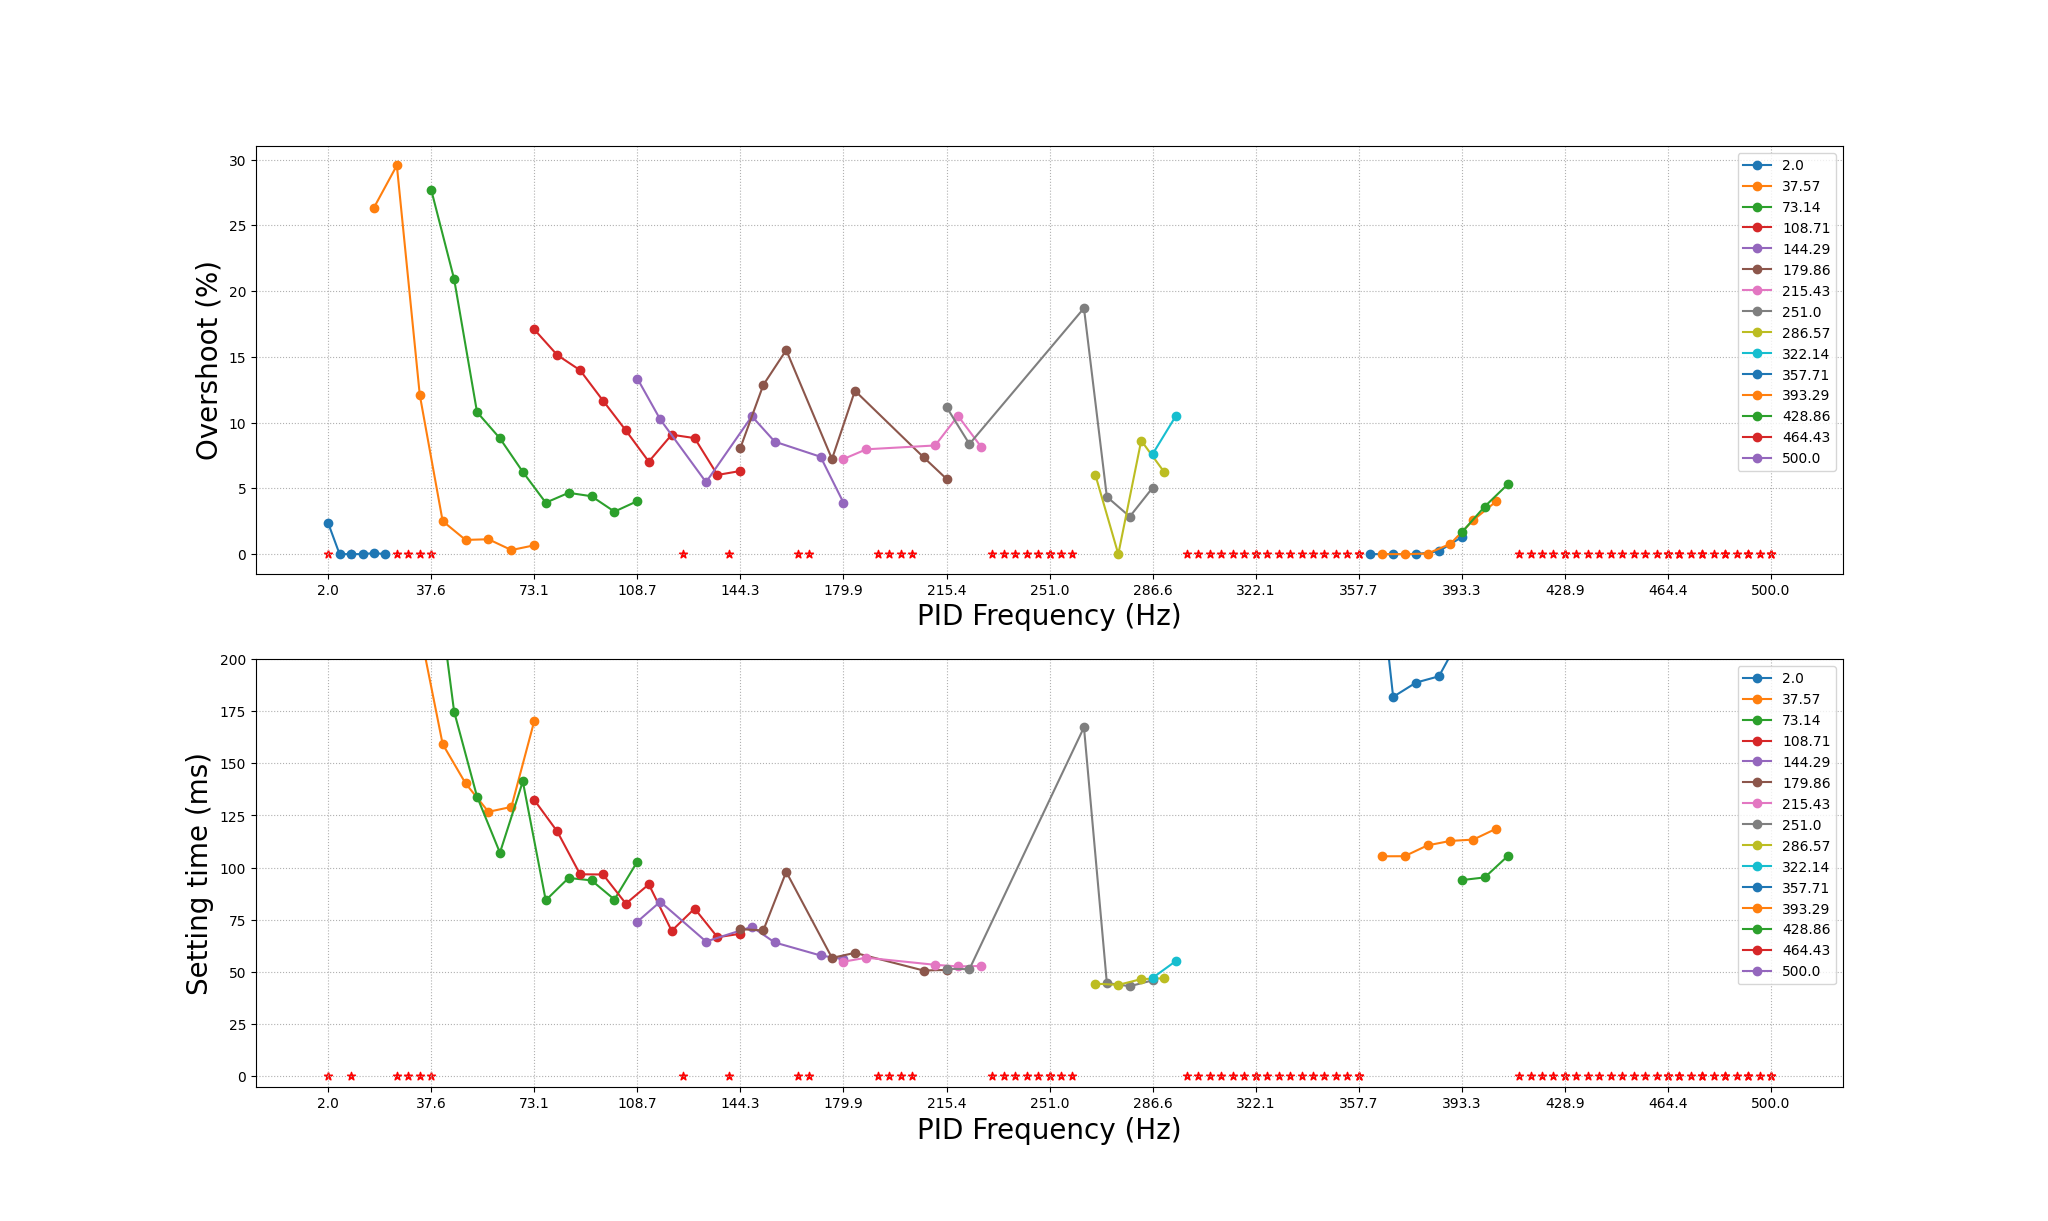
\includegraphics[width=1.3\linewidth]{Report/Pic/Appendix.png}}
\caption{Overall result picture. Red dots represents oscillate.}% 遍历频率域的方法
\label{fig_appendix}
\end{figure}

\end{document}